\section{Implementation}
\label{sec:implementation}

The Django~\cite{django} Web application development framework and the Web API toolkit for Django, Django REST Framework~\cite{drf}, were used to develop our annotation tool.
PostgreSQL~\cite{psql} is used to provide a database for the server-side applications of the software.
This database is responsible for serving the entire data needed to operate the tool, the search API, etc.
During the implementation phase, decisions regarding models in the database have been directed towards making the tool use the API for database queries and searches.
The models reflect the UD format of a sentence and sentences are saved as word lines at the core.

Annotation page has all the functionalities of \boatvone\ and more.
Errors are included for annotators to see invalid edits in real time.
They are checked and annotations validated according to the UD framework and the language provided.
The scripts used for validation are the ones already provided by the framework as of 2022~\cite{UD-git}.

A Python library \textit{spaCy}~\cite{spacy} is used to provide linear dependency graphs.
Another JavaScript-based linear dependency graph~\cite{spyssalo} making use of brat~\cite{brat-vis} is used to provide graphs as well.
The preferences of annotators may vary and giving them options in different parts of the screen is important.

\begin{figure}[tbh]
    \centering
    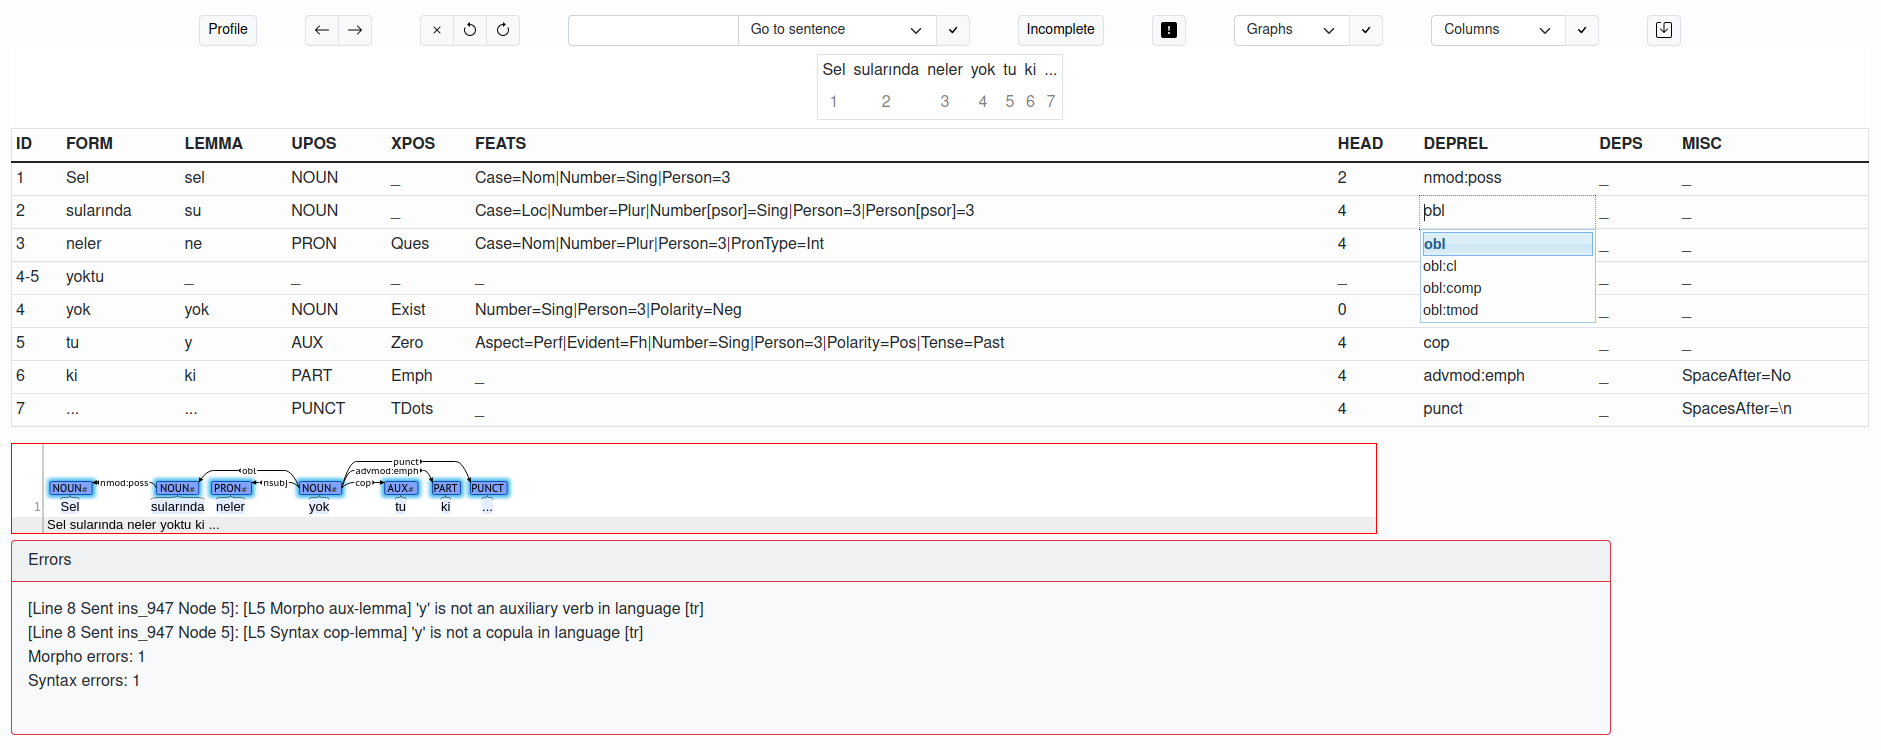
\includegraphics[width=1\textwidth]{figures/1.png}
    \caption{Annotation view for the sentence "Sel sularında neler yoktu ki..."}
    \label{fig:demo-fig}
\end{figure}

\subsection{API}
\label{sec:api}

By using our annotated treebank search API, other parties wanting to see the capabilities of the tool can retrieve our annotated treebanks.
Also, some parties wanting to use the treebanks in their computation tasks can easily extract information from our treebanks by using the API.
This opens up many possibilities for the use of the tool beyond the annotator's UI experience.
We plan to dockerize the tool and make it accessible, following development practices and conventions.

\subsection{New Features}
\label{sec:features}

\section{Features}
\label{sec:features}

There are many new features and improvements in this tool, as well as the functionality that already existed in BoAT v1.
Instead of loading a specific file before annotating, a user is able to upload a \conllu{} file to the database and start annotating.
The file is parsed and checked for its format. It's rejected if incorrectly formatted, then uploaded to the database.
This way, other annotators working for the same treebank don't have to provide the same file.

The annotation page is very similar to BoAT v1.
It includes a dependency graph and an editable table, both of which in sync.
The dependency graph of the initial tool and other 2 graphs have been added to this tool.
The user has the choice to select a type of graph or none.
The other 2 graphs, which are both horizontal and linear, have been selected due to space considerations.
The annotation table is for editing the word lines of \conllu{} files.

An important feature in this version is the ability to cross-check annotations by implementing a network for annotators where they can see the annotations done by other annotators and if they disagree on some parts, they can interact outside the tool.
This can be helpful and a learning experience for annotators.
For an actual example, the annotator, responsible for the BOUN Treebank's annotation, was annotating a sentence that had a Zodiac sign noun.
Not being sure about how to annotate the noun's dependency relation, she searched for similar cases in the \conllu{} file and encountered two different ways nouns of Zodiac signs were annotated previously.
Beside not helping how to choose a \textit{UPOS} tag, this raises a consistency issue within the treebank as well.
For an example of a Turkish sentence with a noun for a Zodiac sign, in the sentence "Terazi rahatına düşkündür." (\textit{"Libras like comfort."}), "Terazi" was annotated as \textit{NOUN} in its \textit{UPOS} tag.
In another sentence "Yükselen Başak düzeni sever." (\textit{"Virgo Rising likes order"}), "Başak" was annotated as \textit{PROPN} in its own \textit{UPOS} tag.
In a similar case, the annotator searched the \conllu{} file in a text editor and decided to use the one with the more cases of annotation and proceeded to replace the inconsistent ones with the decision.
This case can be handled by a simple search of the database.
We provide a search page and its API in this tool where treebanks can be searched by \textit{sent_id}s, \textit{text}s, all the UD tags and treebank names.
With this, an annotator can easily make the treebank more consistent.

% ki example
% Evdeki halılar -> adjectivizer ki 
% Benim halılarım yün, Ayşeninkiler sentetik. -> pronominal 

Also one other thing the interannotator agreement allows us is the possibility to see some anomalies in the Turkish part of the validation of the UD framework.
For example, if a sentence were annotated a way by many annotators but the UD validation script were finding it invalid, this might indicate the UD validation were lacking in this respect of the Turkish language.
Some modifications might be necessary and there could be a case for a proposal of change.

